\documentclass{standalone}
\usepackage{tikz}
\usepackage{pgfplots}
\pgfplotsset{compat=1.17}
\begin{document}

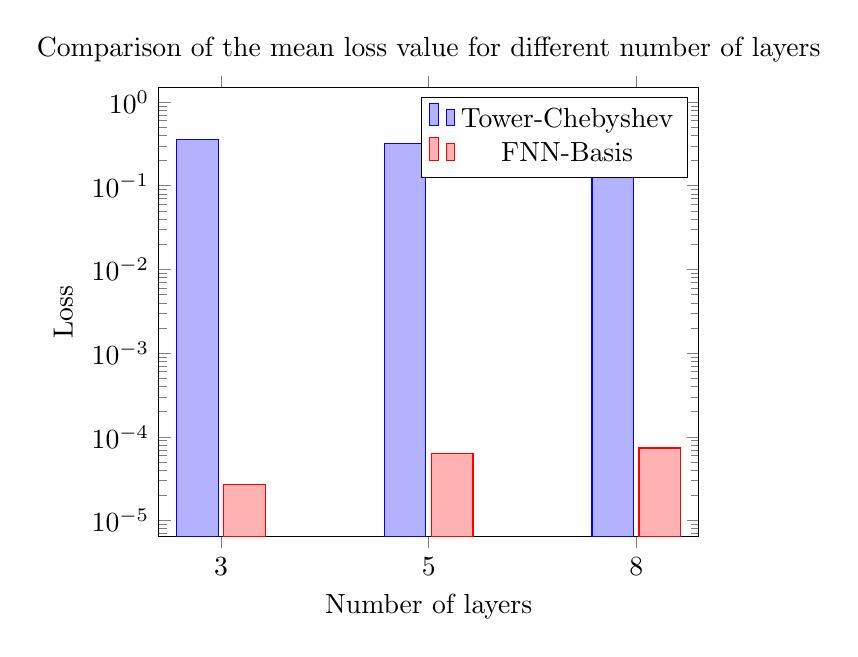
\begin{tikzpicture}
\begin{axis}[
    ybar,
    bar width=15pt,
    enlargelimits=0.15,
    % legend style={at={(0.5,-0.15)}
    % anchor=north,legend columns=-1},
    ylabel={Loss},
    xlabel={Number of layers},
    symbolic x coords={3,5,8},
    xtick=data,
    ymin=0, % Ensure bars start from 0
    title={Comparison of the mean loss value for different number of layers},
    ymode = log,
    log origin=infty,
]
\addplot+[] coordinates {
    (3,0.3559075891971588)
    (5,0.3203471302986145) 
    (8,0.3203469216823578)
};
\addplot+[] coordinates {
    (3,2.7030513592762873e-05) 
    (5,6.306666666666666e-05)
    (8,7.37241207389161e-05)
};
\legend{Tower-Chebyshev, FNN-Basis}
\end{axis}
\end{tikzpicture}

\end{document}
